\texttt{min\_total\_length([1, 2, 3, 7], [0, 4, 5, 9, 10])}

Рисунок ниже иллюстрирует пример.

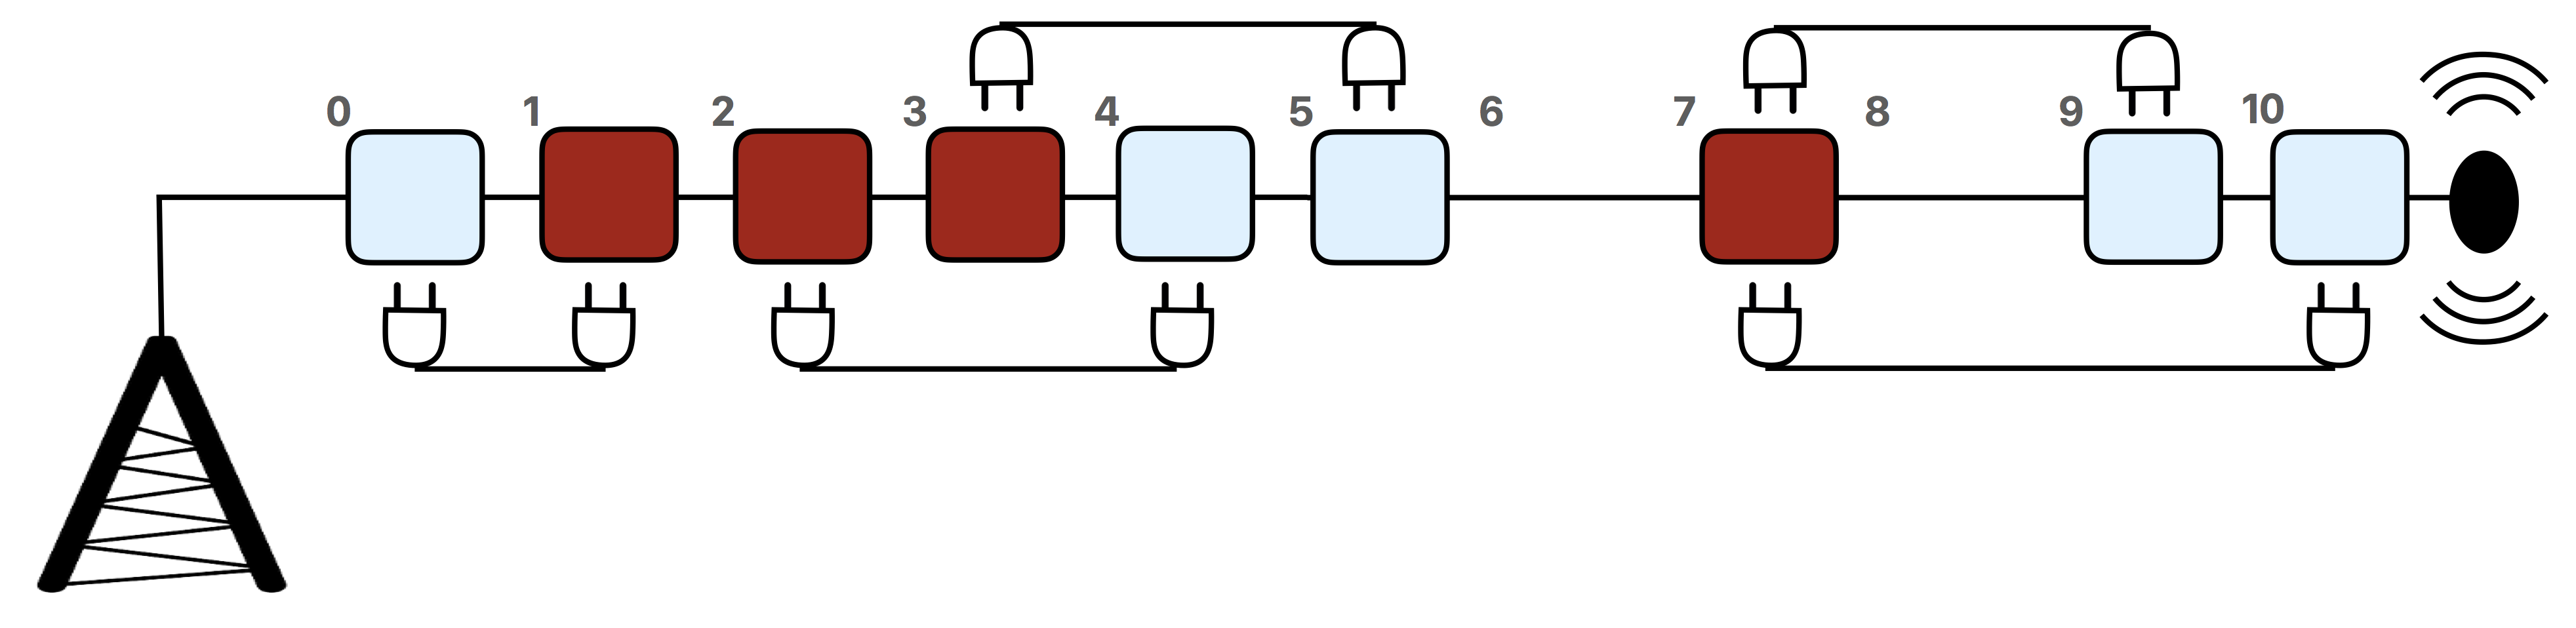
\includegraphics[scale=0.5]{wiring.png}

\begin{itemize}
\item Точки подключения на вышке изображены горизонтально.
\item В чёрно-белой печатной версии красные точки подключения~--- темные, а синие~--- светлые.
\item $4$ красных точки подключения имеют координаты $1, 2, 3,$ и $7$.
\item $5$ синих точек подключения имеют координаты $0, 4, 5, 9,$ и $10$.
\item На рисунке изображена одна из оптимальных схем электропроводки.
\item В этом решении суммарная длина проводов равна $1 + 2 + 2 + 2 + 3 = 10$, и это
значение оптимально. Таким образом, функция должна вернуть значение $10$.
\item Обратите внимание, что два провода соединены с точкой подключения, имеющей
координату $7$.
\end{itemize}